\documentclass{article}\usepackage[]{graphicx}\usepackage[]{color}
%% maxwidth is the original width if it is less than linewidth
%% otherwise use linewidth (to make sure the graphics do not exceed the margin)
\makeatletter
\def\maxwidth{ %
  \ifdim\Gin@nat@width>\linewidth
    \linewidth
  \else
    \Gin@nat@width
  \fi
}
\makeatother

\definecolor{fgcolor}{rgb}{0.345, 0.345, 0.345}
\newcommand{\hlnum}[1]{\textcolor[rgb]{0.686,0.059,0.569}{#1}}%
\newcommand{\hlstr}[1]{\textcolor[rgb]{0.192,0.494,0.8}{#1}}%
\newcommand{\hlcom}[1]{\textcolor[rgb]{0.678,0.584,0.686}{\textit{#1}}}%
\newcommand{\hlopt}[1]{\textcolor[rgb]{0,0,0}{#1}}%
\newcommand{\hlstd}[1]{\textcolor[rgb]{0.345,0.345,0.345}{#1}}%
\newcommand{\hlkwa}[1]{\textcolor[rgb]{0.161,0.373,0.58}{\textbf{#1}}}%
\newcommand{\hlkwb}[1]{\textcolor[rgb]{0.69,0.353,0.396}{#1}}%
\newcommand{\hlkwc}[1]{\textcolor[rgb]{0.333,0.667,0.333}{#1}}%
\newcommand{\hlkwd}[1]{\textcolor[rgb]{0.737,0.353,0.396}{\textbf{#1}}}%

\usepackage{framed}
\makeatletter
\newenvironment{kframe}{%
 \def\at@end@of@kframe{}%
 \ifinner\ifhmode%
  \def\at@end@of@kframe{\end{minipage}}%
  \begin{minipage}{\columnwidth}%
 \fi\fi%
 \def\FrameCommand##1{\hskip\@totalleftmargin \hskip-\fboxsep
 \colorbox{shadecolor}{##1}\hskip-\fboxsep
     % There is no \\@totalrightmargin, so:
     \hskip-\linewidth \hskip-\@totalleftmargin \hskip\columnwidth}%
 \MakeFramed {\advance\hsize-\width
   \@totalleftmargin\z@ \linewidth\hsize
   \@setminipage}}%
 {\par\unskip\endMakeFramed%
 \at@end@of@kframe}
\makeatother

\definecolor{shadecolor}{rgb}{.97, .97, .97}
\definecolor{messagecolor}{rgb}{0, 0, 0}
\definecolor{warningcolor}{rgb}{1, 0, 1}
\definecolor{errorcolor}{rgb}{1, 0, 0}
\newenvironment{knitrout}{}{} % an empty environment to be redefined in TeX

\usepackage{alltt}

\usepackage[brazilian]{babel}
\usepackage[utf8]{inputenc}
\usepackage[T1]{fontenc}
\usepackage{indentfirst}
\IfFileExists{upquote.sty}{\usepackage{upquote}}{}
\begin{document}

\title{Desigualdades socioeconômicas nos EUA na década de 90}
\author{Caio C. C. Dias \\ \texttt{7557720}}
\maketitle



\section{Introdução}
\par Em 1950, o  escritor Nelson Rodrigues cunhou a expressão ``Complexo de vira-lata'' para entitular a inferioridade que o brasileiro se coloca em face do resto do mundo. Tal complexo nos acompanha até hoje e é muito comum escutar-se bordões como: ``se fosse em outro país, a coisa seria diferente!''. Talvez, devido a proximidade geográfica e o título de maior potência mundial, este ``outro país'' é comumente os Estados Unidos.
\par Este trabalho, tem por objetivo analisar dados abertos de um recenseamento feito nos EUA em 1994 e assim demonstrar que, ao menos, os EUA também demonstravam uma grande desigualdade sócioeconômica em 1994.

\section{Análises}
\par Na primeira figura, alguns dados relevantes foram cruzados com os dados saláriais, assim, podemos traçar um perfil de como são as pessoas que ganham mais de 50.000 USD por ano. De forma resumida, podemos dizer que as pessoas que ganham mais dinheiro são mais velhas, possuem mais anos de escolaridade, são casadas, a posição familiar é a de marido, etnia branca e gênero masculino.
\par Já na segunda figura, podemos notar aonde a relação horas trabalhadas por semana versus idade tem sua maior densidade.

\begin{knitrout}
\definecolor{shadecolor}{rgb}{0.969, 0.969, 0.969}\color{fgcolor}
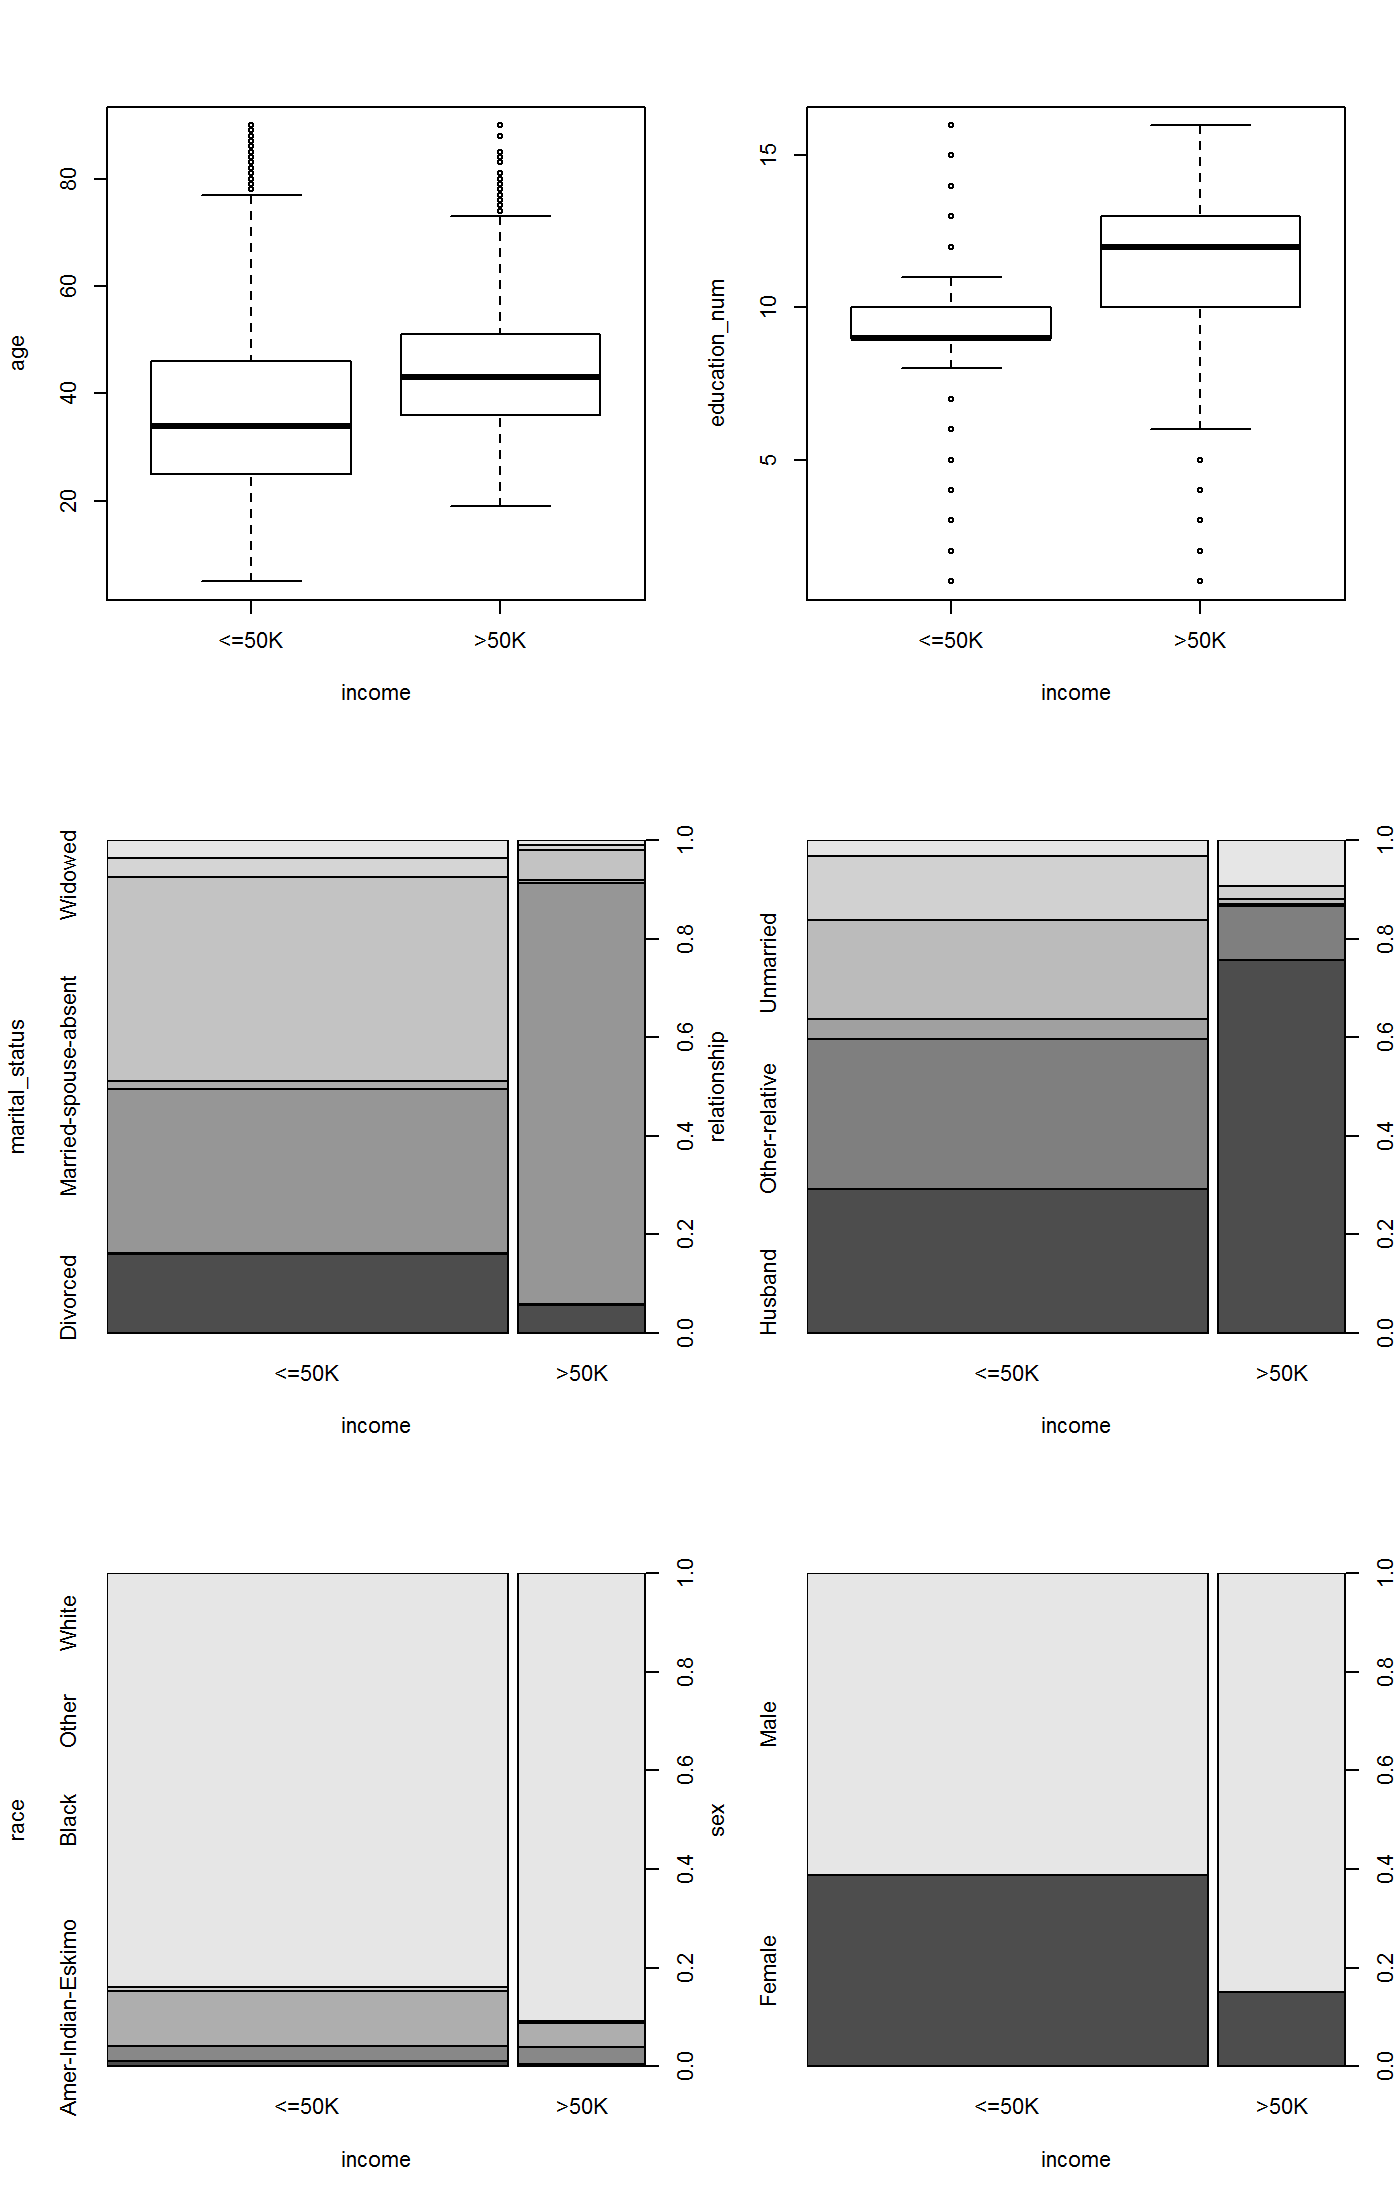
\includegraphics[width=\maxwidth]{figure/generalanalysis-1} 

\end{knitrout}

\begin{knitrout}
\definecolor{shadecolor}{rgb}{0.969, 0.969, 0.969}\color{fgcolor}
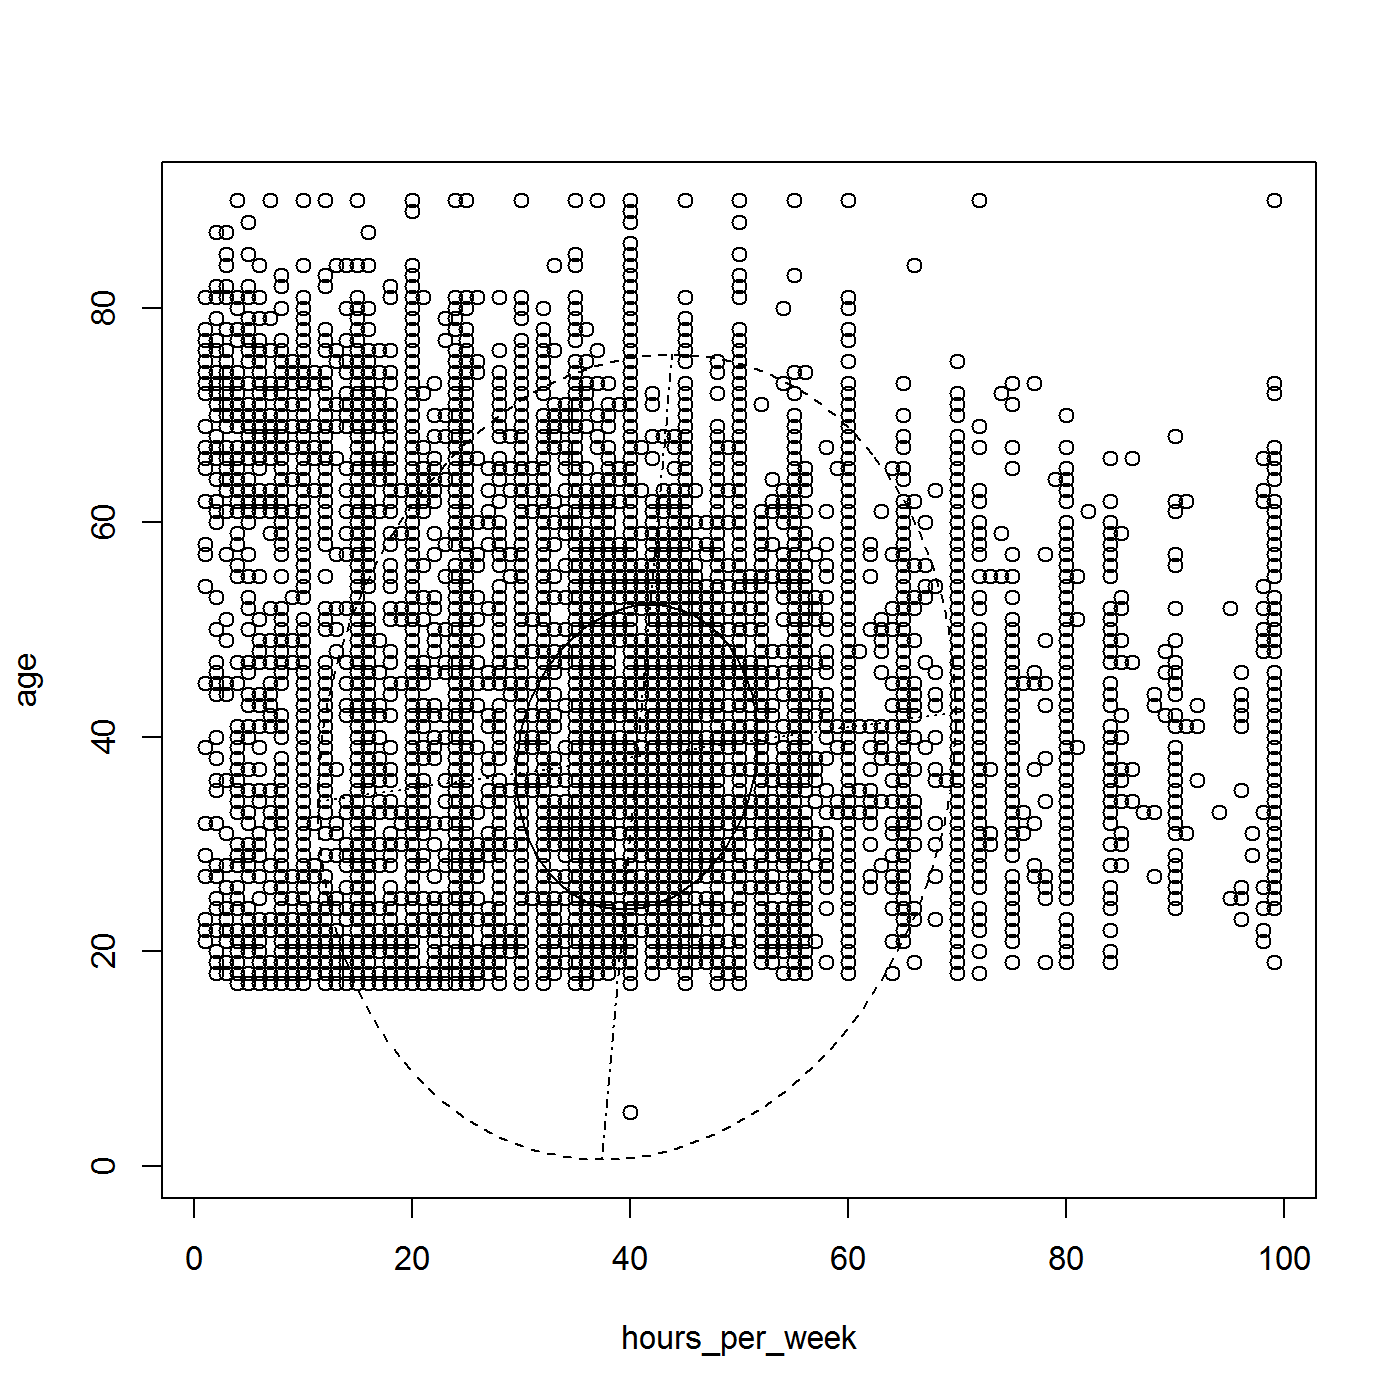
\includegraphics[width=\maxwidth]{figure/agehours-1} 

\end{knitrout}

\section{Provas de Conceito}
\par Já esta seção, contém apenas gráficos para demonstrar o uso de algumas funções, pois não podem serem aplicadas a esta análise gerando resultados interessantes.
\par Dentre as técnicas aqui utilizadas temos \texttt{qqplot}, \texttt{rug}, \texttt{hull} e \texttt{polygon}.

\begin{knitrout}
\definecolor{shadecolor}{rgb}{0.969, 0.969, 0.969}\color{fgcolor}
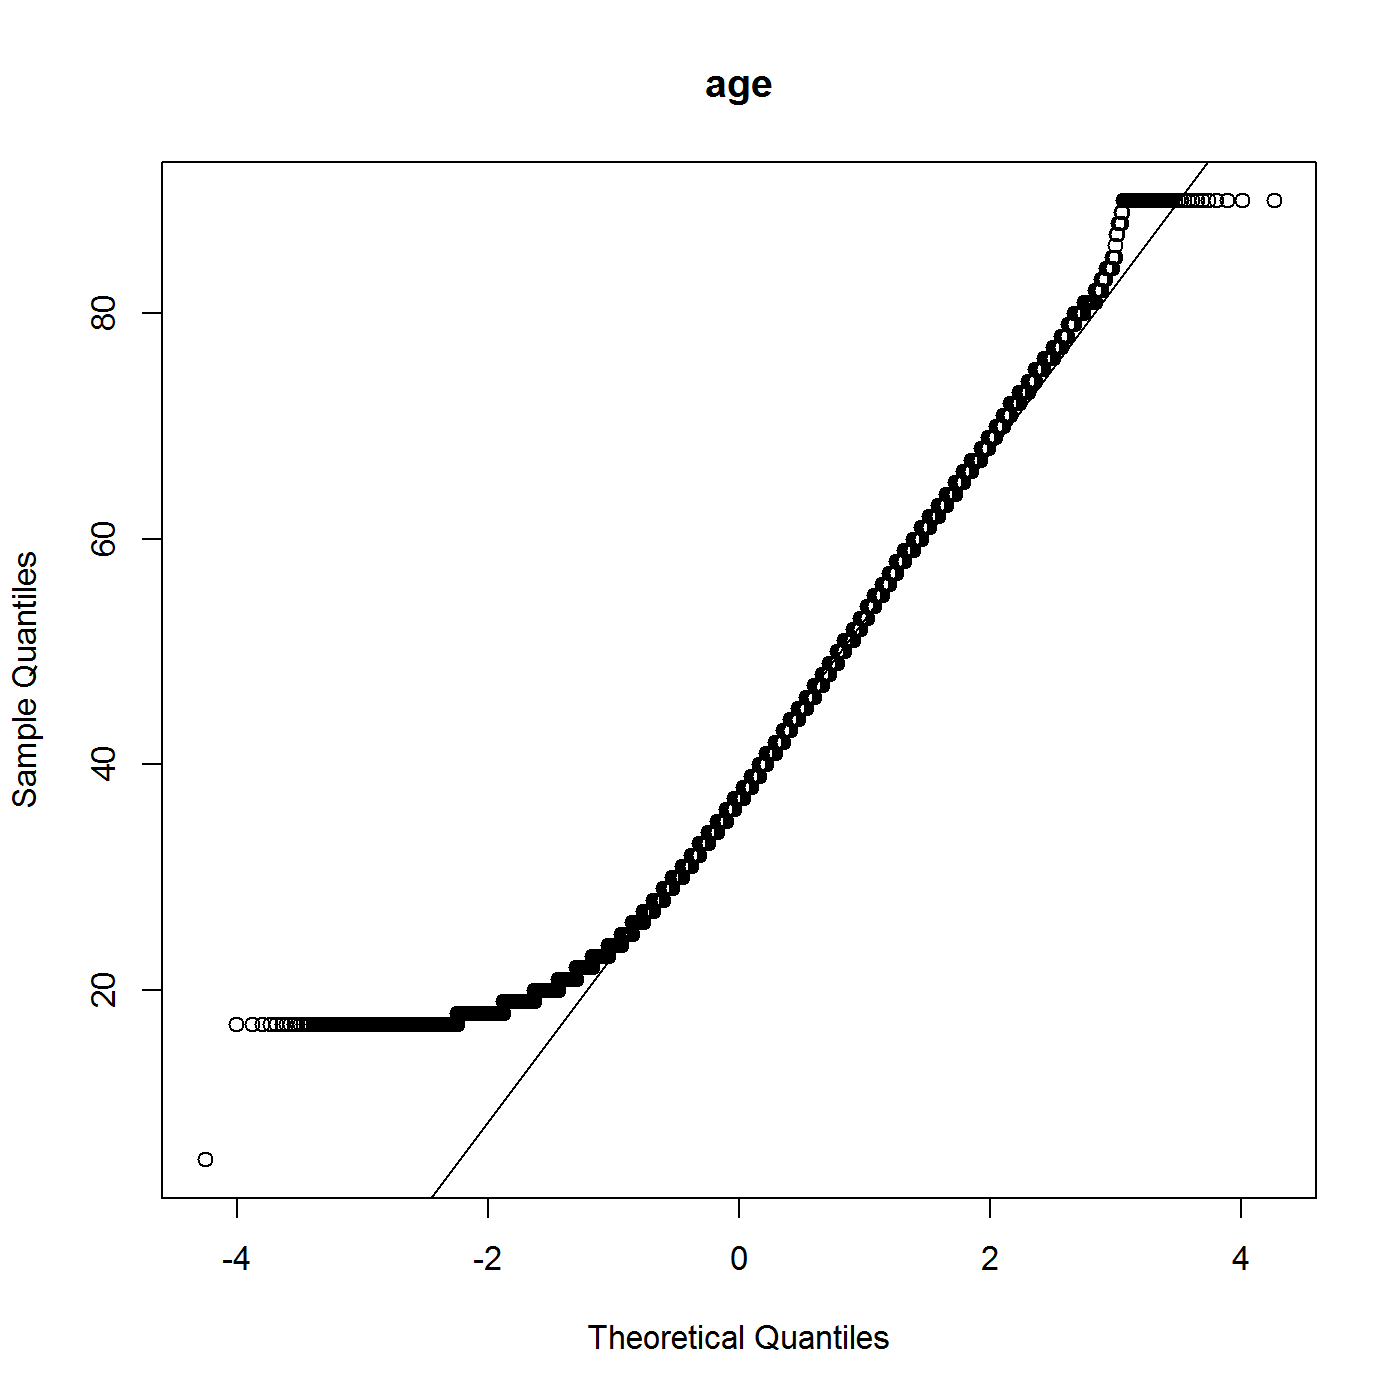
\includegraphics[width=\maxwidth]{figure/qqplot-1} 

\end{knitrout}

\begin{knitrout}
\definecolor{shadecolor}{rgb}{0.969, 0.969, 0.969}\color{fgcolor}
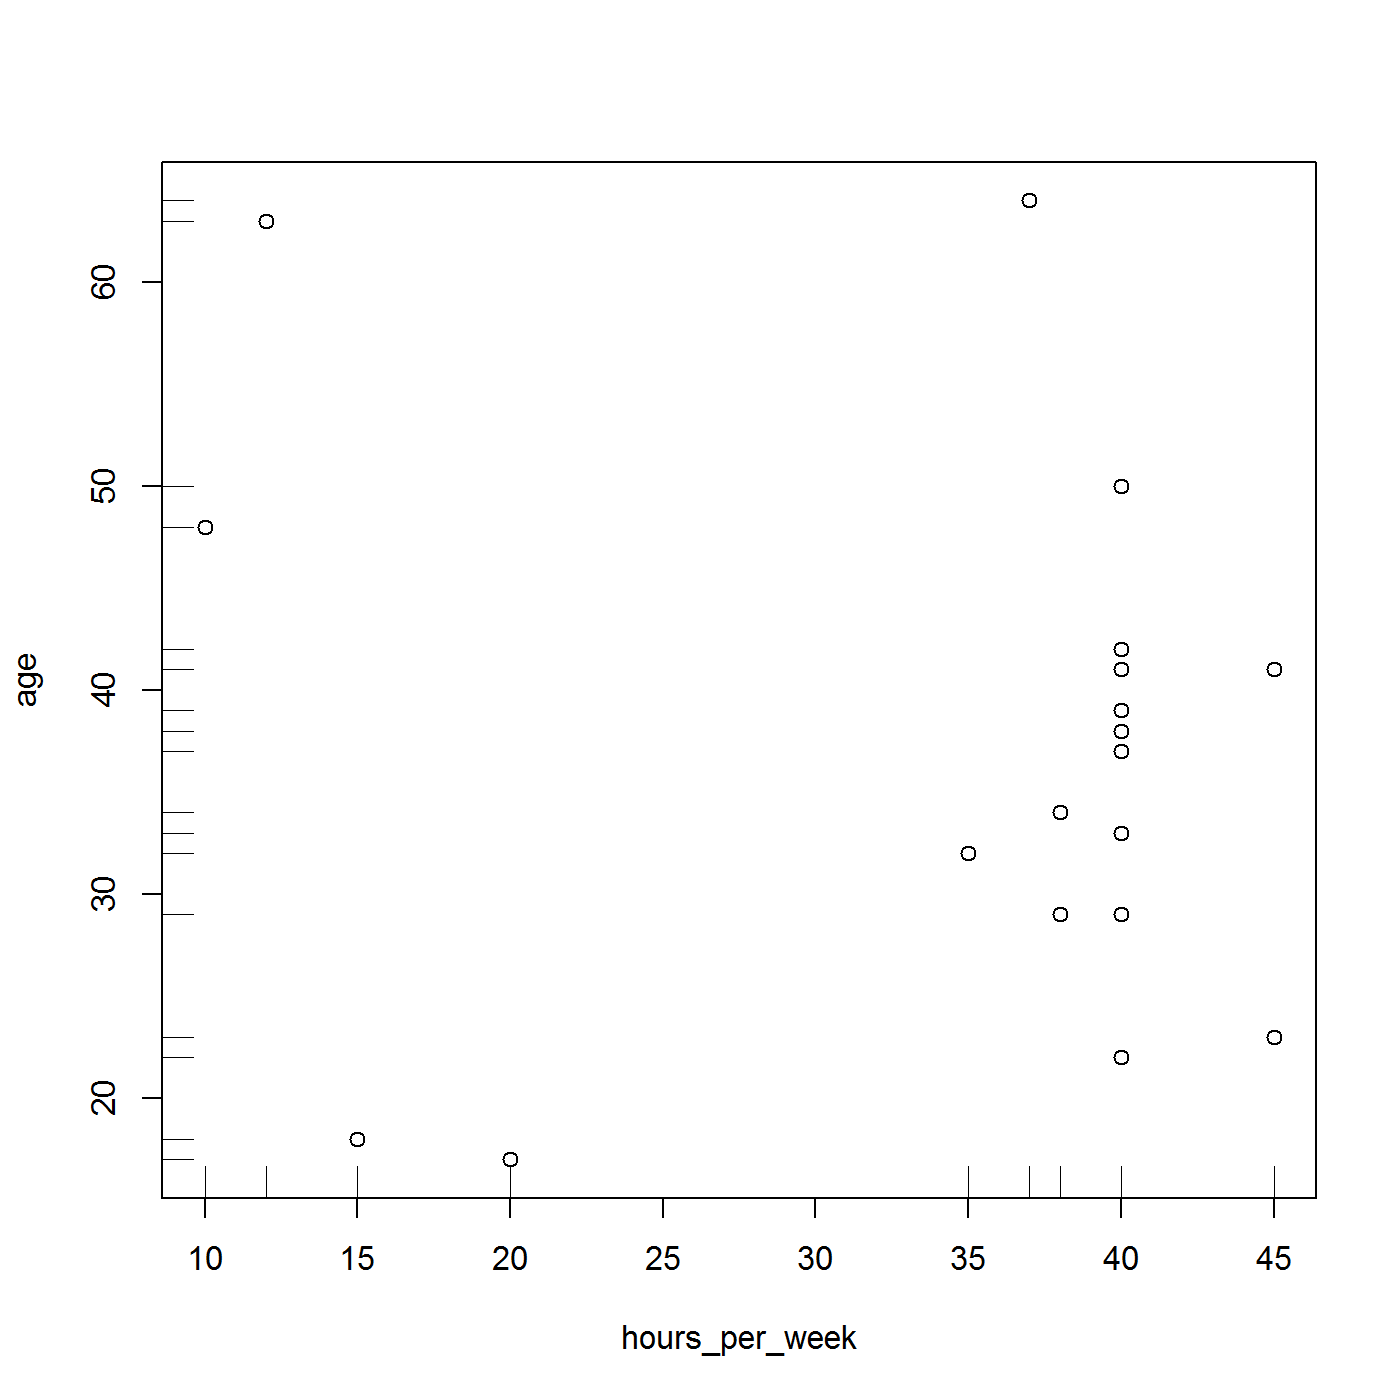
\includegraphics[width=\maxwidth]{figure/rug-1} 

\end{knitrout}

\begin{knitrout}
\definecolor{shadecolor}{rgb}{0.969, 0.969, 0.969}\color{fgcolor}
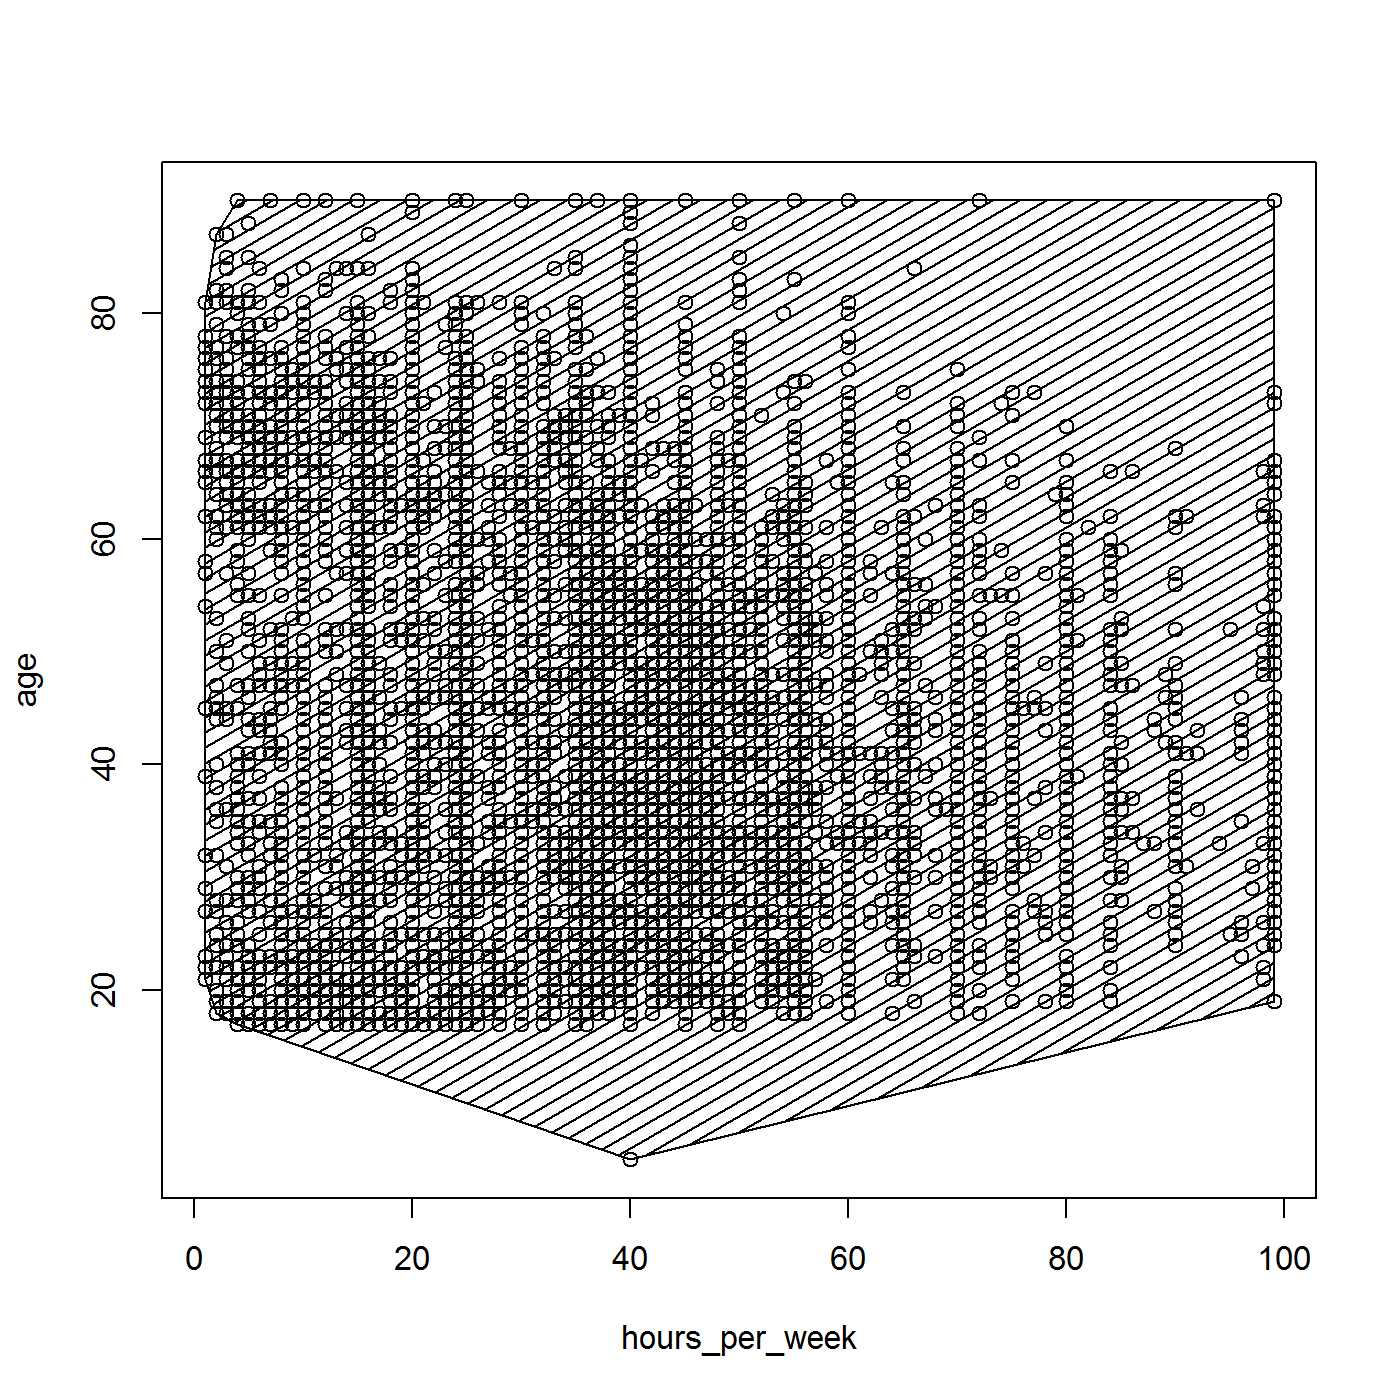
\includegraphics[width=\maxwidth]{figure/hullpolygon-1} 

\end{knitrout}

\begin{knitrout}
\definecolor{shadecolor}{rgb}{0.969, 0.969, 0.969}\color{fgcolor}
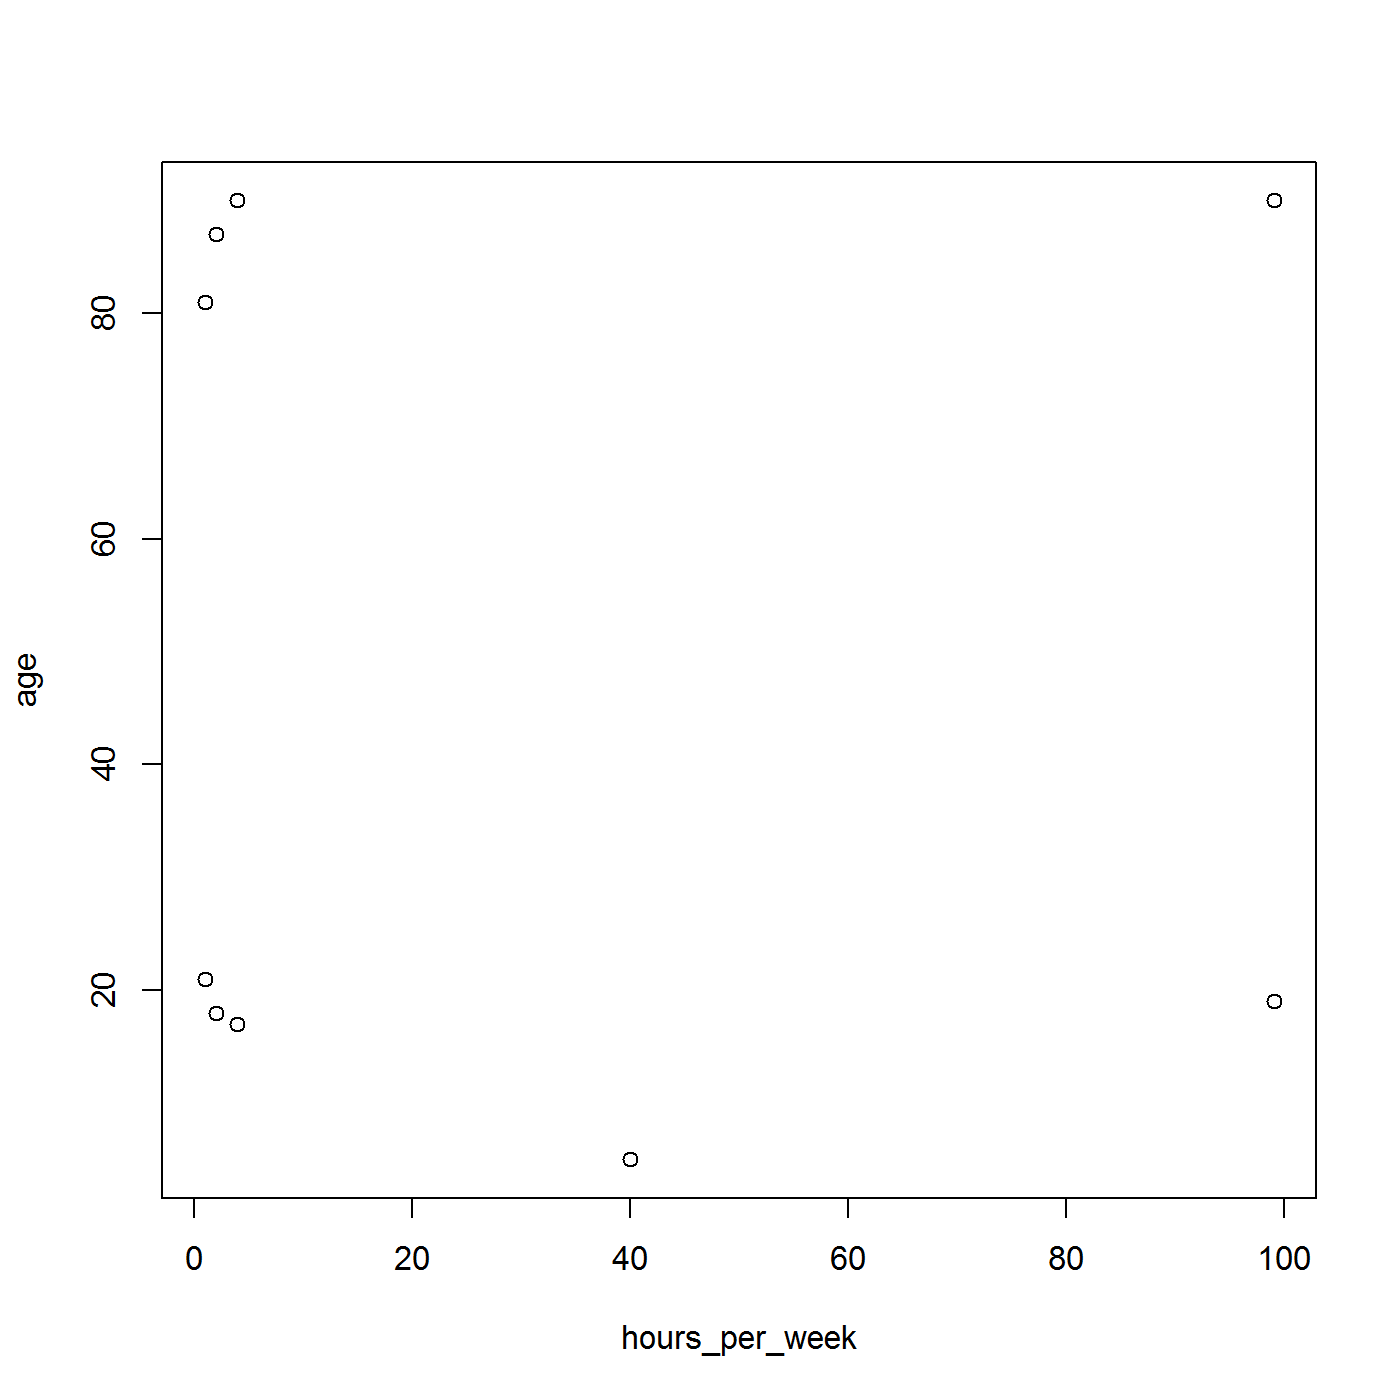
\includegraphics[width=\maxwidth]{figure/onlyhull-1} 

\end{knitrout}

\end{document}
